\section{Cliente}

\subsection{Header}

\begin{figure}[htbp]
    \centering
	
\includegraphics[width=0.8\textwidth]{PB/manuale-utente/header-cliente.png}
    \caption{Barra di Navigazione per il cliente}
\end{figure}

La barra di navigazione in alto ti permette di accedere facilmente alle varie 
sezioni della piattaforma:
\begin{itemize}
	\item \texttt{Logo e "Easy Meal"}: cliccando sul logo o sul nome "Easy Meal"
		sei reindirizzato alla Home Page della piattaforma;

	\item \texttt{Esplora}: cliccando su questo riferimento sei reindirizzato
		alla Home Page della piattaforma;

	\item \texttt{Prenotazioni}: cliccando su questo riferimento sei 
		reindirizzato alla pagina di visualizzazione della lista di
		prenotazioni;

	\item \texttt{Notifiche}: cliccando su questo riferimento sei reindirizzato
		alla pagina di visualizzazione della lista di notifiche. Nota che se ci
		sono notifiche non lette, il riferimento sarà seguito da un badge che
		indica il numero di notifiche non lette;

	\item \texttt{Logout}: cliccando su questo riferimento effettuerai il \textit{logout}
		dalla piattaforma e sarai reindirizzato alla Home Page della 
		piattaforma.
\end{itemize}

\subsection{Home Page}

La Home Page del cliente è analoga a quella dell'utente non autenticato, cambia
solamente l'\textit{header}.

\subsection{Visualizza in dettaglio un ristorante}

\begin{figure}[htbp]
    \centering
	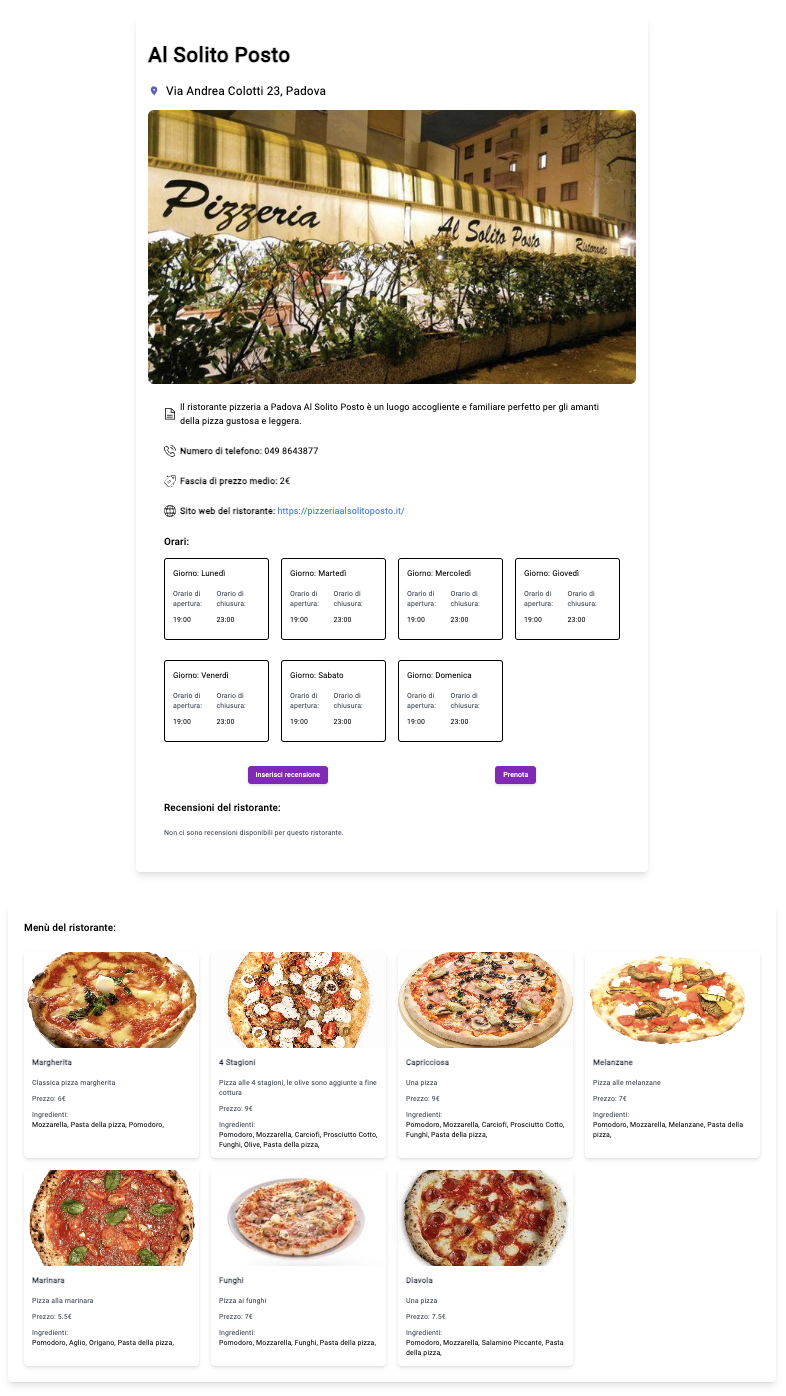
\includegraphics[width=0.6\textwidth]{PB/manuale-utente/dettagli-ristorante-cliente.png}
    \caption{Pagina di visualizzazione in dettaglio di un ristorante per il
	cliente}
\end{figure}
\newpage
Questa pagina è analoga a quella dell'utente non autenticato, ci sono tuttavia
due aggiunte:
\begin{itemize}
	\item \texttt{Inserisci recensione}: questo bottone compare in mezzo tra le
		gli orari di apertura di un ristorante e le sue recensioni, accanto al
		pulsante qui sotto. Cliccando su questo bottone si viene reindirizzati
		ad una pagina in cui è possibile inserire una recensione per il
		ristorante. Questo bottone compare solo se si è conclusa una
		prenotazione e quindi si ha effetuato un pagamento presso il ristorante e non si è ancora inserita una
		recensione;

	\item \texttt{Prenota}: questo bottone si trova sotto gli orari del
		ristorante. Cliccando su questo bottone si viene reindirizzati alla
		pagina di prenotazione di un tavolo presso il ristorante che si sta
		visualizzando.
\end{itemize}

\subsection{Prenotazione di un tavolo}

\begin{figure}[htbp]
    \centering
	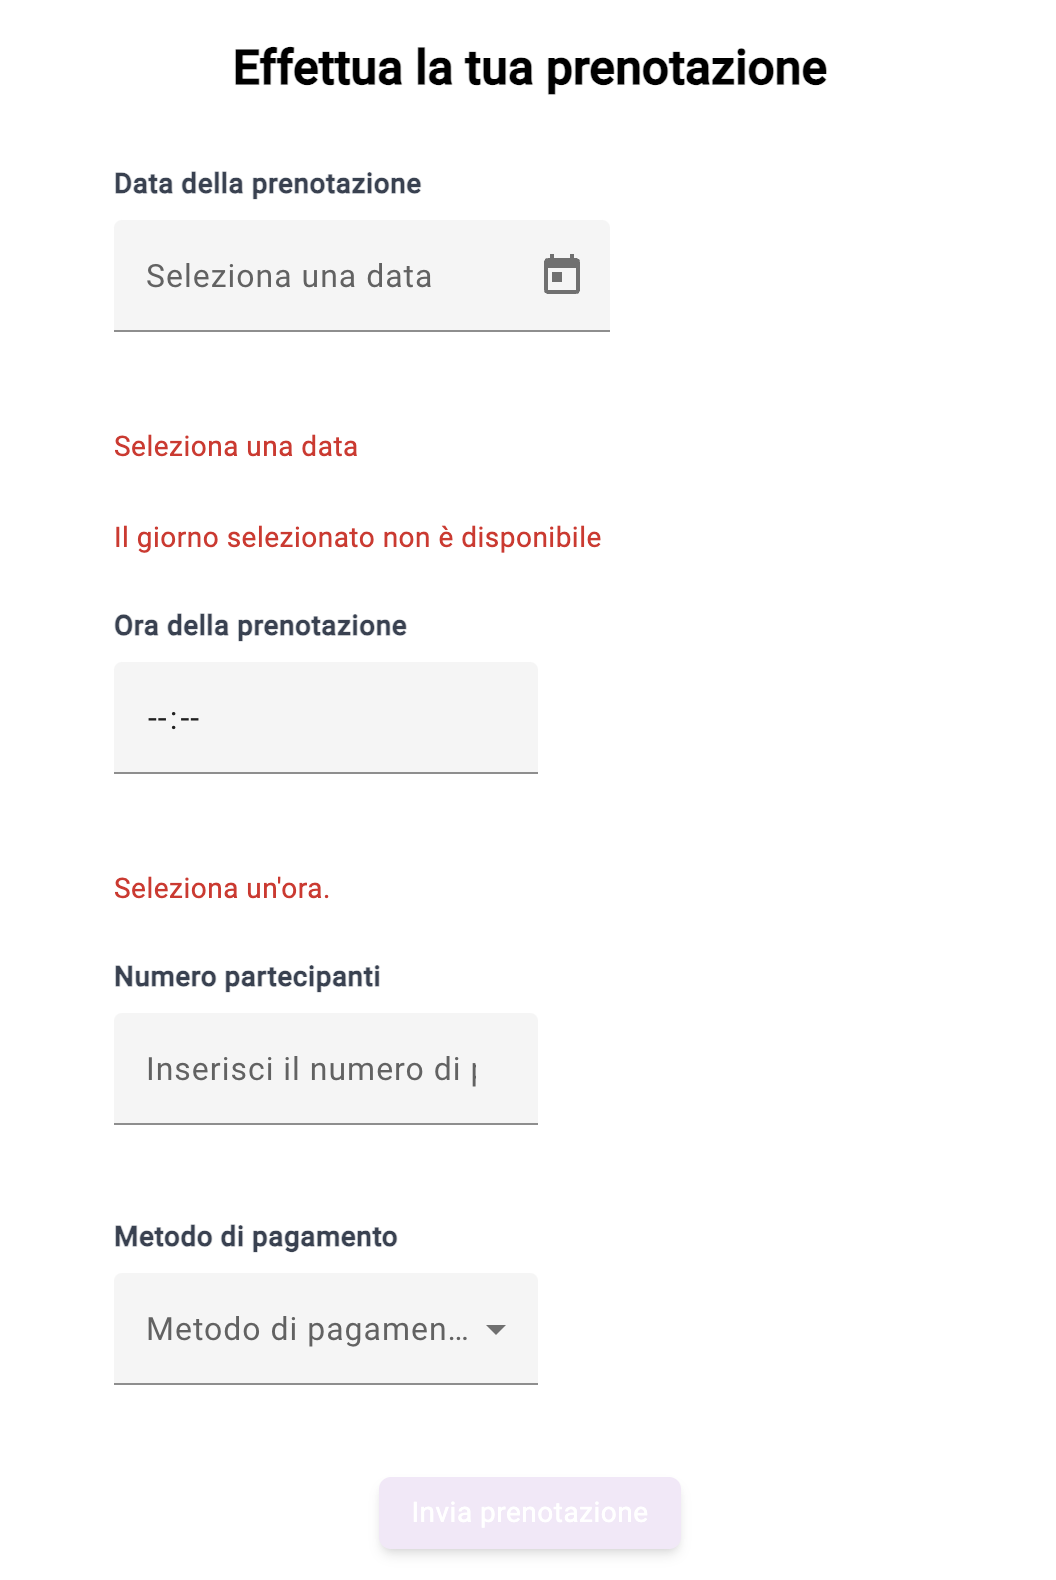
\includegraphics[width=0.4\textwidth]{PB/manuale-utente/prenotazione.png}
    \caption{Pagina di richiesta di una prenotazione per il cliente}
\end{figure}

Si accede a questa pagina cliccando sul bottone \texttt{Prenota} della pagina di
dettaglio di un ristorante. Dopo aver compilato il \textit{form} con le informazioni
richieste:
\begin{itemize}
	\item Data della prenotazione: viene richiesto di inserire la data in cui si
		vuole prenotare il tavolo nel formato \texttt{mm/gg/aaaa}. Accanto al
		\textit{form} di inserimento è presente il bottone di un calendario che apre un
		calendario con i giorni. Cliccando su un giorno del calendario, il \textit{form}
		viene automaticamente compilato con la data selezionata;

	\item Ora della prenotazione: viene richiesto di inserire l'orario in cui si
		vuole prenotare il tavolo nel formato \texttt{hh:mm}. Sono accettati
		solamente orari compresi all'interno degli orari di apertura del
		ristorante presso cui si desidera prenotare;

	\item Numero partecipanti: con un numero di partecipanti maggiore di 1
		appaiono dei campi aggiuntivi per inserire le \textit{email} dei partecipanti
		supplementari, in questo modo è possibile condividere la prenotazione
		con altri utenti;

	\item Metodo di pagamento: si può scegliere di pagare in modo equidiviso
		(alla "romana") oppure di pagare in modo individuale, e quindi ciascun
		partecipante paga solo per se stesso.
\end{itemize}

Dopo aver compilato il \textit{form}, cliccando sul bottone \texttt{Invia prenotazione} 
si richiede la prenotazione del tavolo. Se la richiesta è andata a buon fine
viene visualizzato un messaggio di successo e si è reindirizzati alla pagina di
visualizzazione della lista di prenotazioni; altrimenti viene visualizzato un
messaggio di errore.

\newpage
\subsection{Lista delle prenotazioni}
\begin{figure}[htbp]
    \centering
	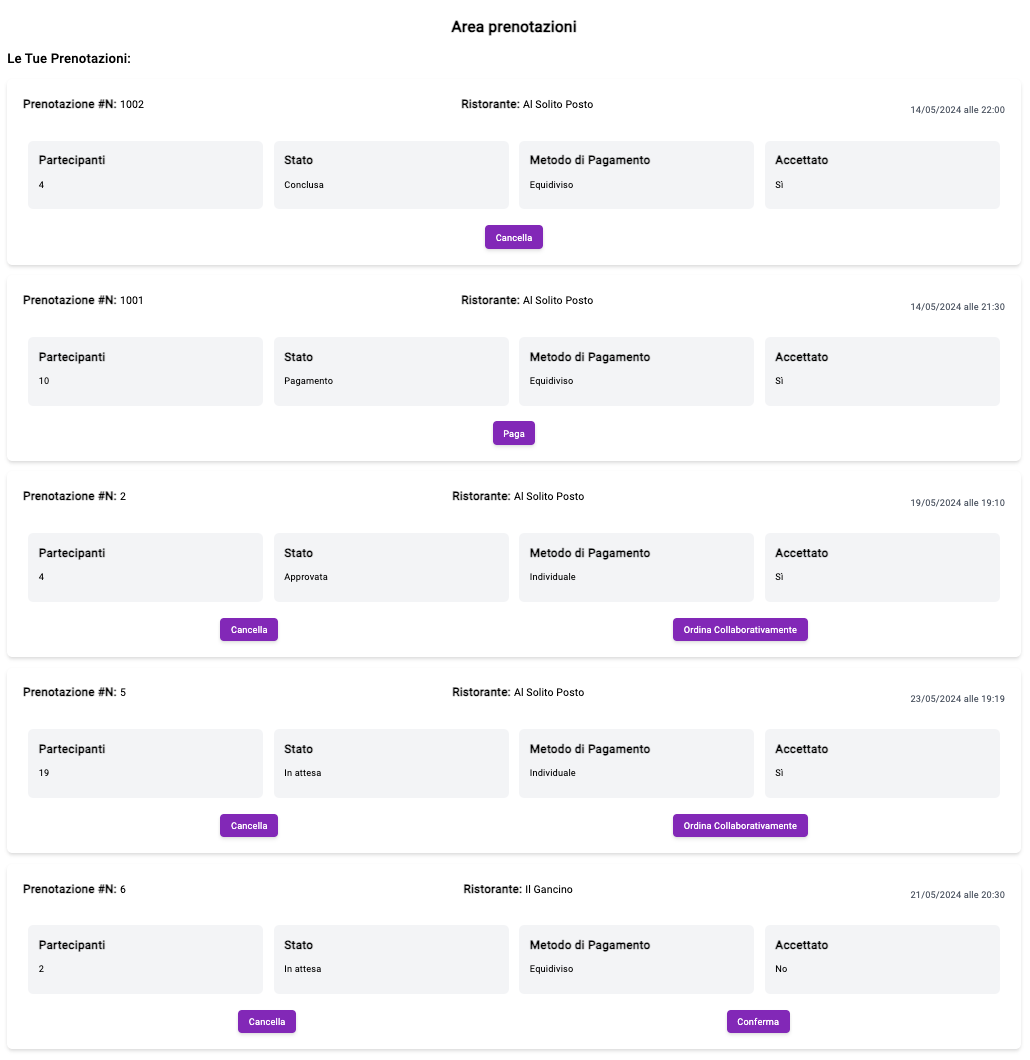
\includegraphics[width=0.8\textwidth]{PB/manuale-utente/lista-prenotazioni-cliente.png}
    \caption{Pagina di visualizzazione delle prenotazioni per il cliente}
\end{figure}

Si può accedere a questa pagina cliccando sul bottone \texttt{Prenotazioni} della
barra di navigazione. In questa pagina sono visualizzate tutte le prenotazioni
di un cliente. In particolare a seconda dello stato della prenotazione sono
possibili diverse operazioni sulle prenotazioni:
\begin{itemize}
	\item \textbf{"In Attesa"} oppure \textbf{"Approvata"}: 
		\begin{itemize}
			\item \texttt{Cancella}: la prenotazione è annullata per te
				(se una prenotazione è condivisa, la cancellazione della
				prenotazione avviene solo quando tutti i partecipanti hanno cancellato
				la prenotazione). Questa operazione cancella la prenotazione
				dalla lista delle prenotazioni del cliente;

			\item \texttt{Ordina collaborativamente}: cliccando su questo
				bottone si viene reindirizzati alla pagina di gestione delle
				ordinazioni collegate alla prenotazione selezionate.
		\end{itemize}

	\item \textbf{"Pagamento"}: 
		\begin{itemize}
			\item \texttt{Paga}: cliccando su questo bottone si viene
				reindirizzati alla pagina di pagamento della prenotazione
				selezionata.
		\end{itemize}

	\item \textbf{"Conclusa"} oppure \textbf{"Rifiutata"}: 
		\begin{itemize}
			\item \texttt{Cancella}: la prenotazione viene non sarà più visibile
				nella lista delle prenotazioni del cliente.
		\end{itemize}

	\item \textbf{Accettato: No}: si tratta di un invito a partecipare ad una
		prenotazione condivisa.
		\begin{itemize}
			\item \texttt{Conferma}: cliccando su questo bottone si accetta la
				prenotazione selezionata;

			\item \texttt{Cancella}: cliccando su questo bottone si rifiuta la
				prenotazione selezionata.
		\end{itemize}
\end{itemize}

\newpage
\subsection{Ordinazione collaborativa}

\begin{figure}[htbp]
	\centering
	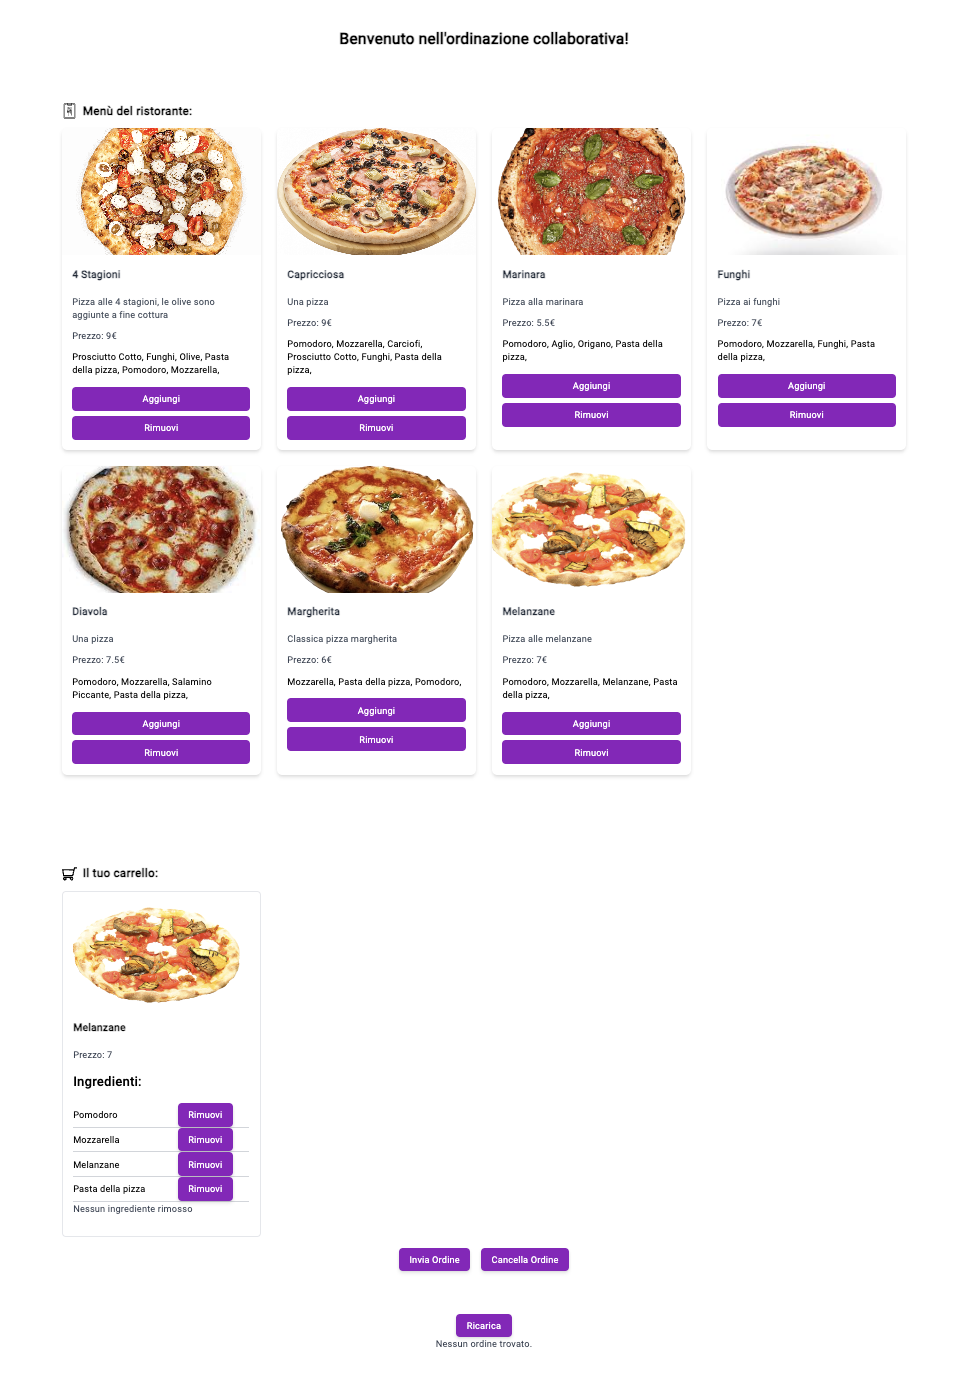
\includegraphics[width=0.77\textwidth]{./img/menu-ordinazione-collaborativa.png}
	\caption{Pagina del menù dell'ordinazione collaborativa}
 \end{figure}
 \newpage
La funzionalità di \textit{ordinazione collaborativa} permette ai clienti di effettuare ordini in modo collettivo, facilitando la gestione delle prenotazioni di gruppo. 
Quando un cliente preme il bottone \texttt{Ordina collaborativamente} presente nella lista delle prenotazioni, viene reindirizzato alla pagina dell'ordinazione 
collaborativa, dove viene visualizzato il menù del ristorante scelto.

All'interno del menù, per ogni piatto vengono mostrate le seguenti informazioni:
\begin{itemize}
    \item \textbf{Nome del piatto}: il nome identificativo del piatto.
    \item \textbf{Immagine del piatto}: una rappresentazione visiva del piatto.
    \item \textbf{Prezzo}: il costo del piatto.
    \item \textbf{Ingredienti}: una lista dettagliata di tutti gli ingredienti presenti nel piatto.
\end{itemize}

Gli utenti possono interagire con ogni piatto presente nel menù utilizzando due bottoni:
\begin{itemize}
    \item \texttt{Aggiungi}: aggiunge il piatto selezionato al carrello del cliente.
    \item \texttt{Rimuovi}: rimuove il piatto selezionato dal carrello del cliente.
\end{itemize}

Il carrello del cliente viene visualizzato subito sotto il menù del ristorante, permettendo al cliente di vedere in ogni momento lo stato del proprio carrello. 
Nel carrello sono elencati tutti i piatti aggiunti per l'ordinazione corrente. Per ciascun piatto nel carrello, l'utente ha la possibilità di personalizzare ulteriormente 
l'ordine:
\begin{itemize}
    \item \texttt{Rimuovi ingrediente}: affianco ad ogni ingrediente è presente un bottone \texttt{Rimuovi} che, se premuto, rimuove l'ingrediente specifico dal piatto.
\end{itemize}

Quando il cliente ha terminato di comporre il suo ordine, ha a disposizione due opzioni:
\begin{itemize}
    \item \texttt{Invia ordine}: invia l'ordine corrente, rendendolo definitivo.
    \item \texttt{Cancella Ordine}: cancella l'ordine del cliente soltanto se è già stato inviato, rimuovendo l'ordine dalla ordinazione collaborativa.
\end{itemize}

Se il cliente desidera modificare la propria ordinazione, può farlo in due modi:
\begin{itemize}
    \item \textbf{Cancellare e ricreare}: può cancellare l'ordinazione precedente premendo il bottone \texttt{Cancella Ordine} e poi creare una nuova ordinazione 
	con le modifiche desiderate.
    \item \textbf{Sovrascrivere}: può semplicemente aggiungere o rimuovere piatti e ingredienti dal carrello e poi premere il bottone \texttt{Invia ordine} 
	per sovrascrivere l'ordine precedente con quello nuovo.
\end{itemize}


In fondo alla pagina dell'ordinazione collaborativa, vengono visualizzati tutti gli ordini effettuati dagli altri commensali che partecipano alla stessa prenotazione 
del cliente, oltre all'ordine del cliente stesso. Questa funzionalità permette di monitorare gli ordini degli altri partecipanti, facilitando la gestione delle ordinazioni 
di gruppo. Ogni ordine è accompagnato dal nome del commensale che lo ha effettuato.
In fondo alla pagina è presente un bottone \texttt{Ricarica} che, se premuto, aggiorna la lista degli ordini, mostrando la lista più recente di tutti gli ordini effettuati.


\subsection{Pagamento di una prenotazione}
\begin{figure}[htbp]
    \centering
	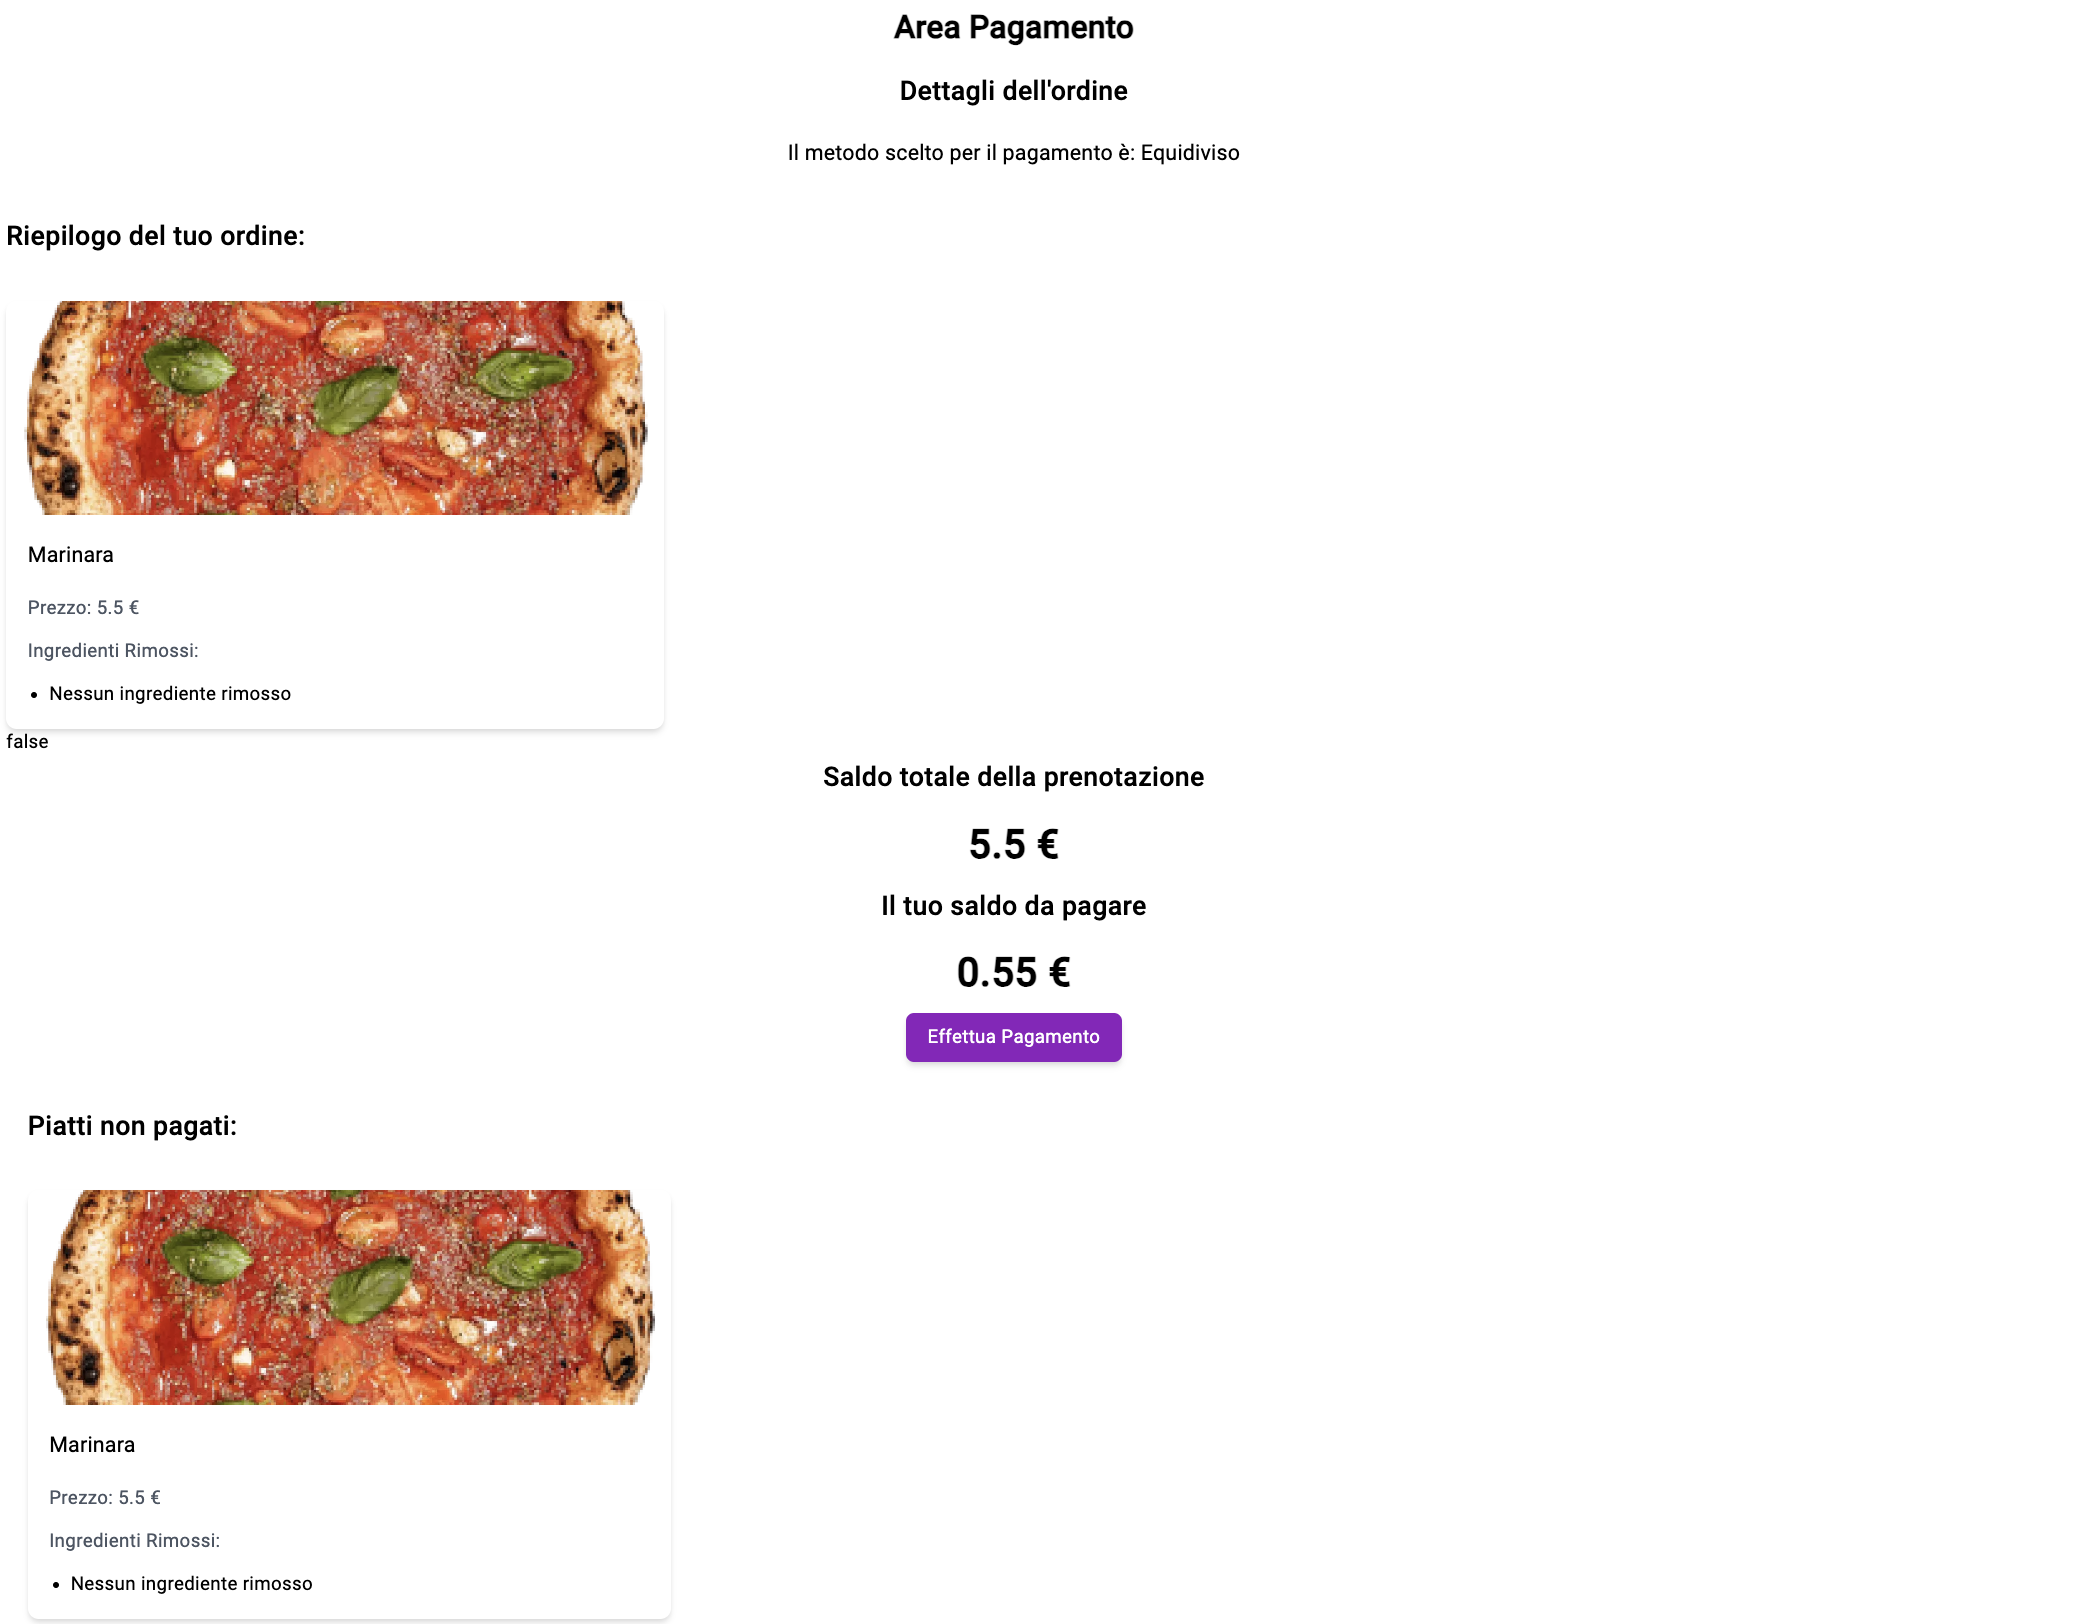
\includegraphics[width=0.8\textwidth]{PB/manuale-utente/pagamento.png}
    \caption{Pagina di pagamento di una prenotazione}
\end{figure}

Si accede a questa pagina cliccando sul bottone \texttt{Paga} della pagina di
visualizzazione delle prenotazioni, se la prenotazione è in stato "Pagamento".
In questa pagina è mostrato il riepilogo degli ordini effettuati, il totale da
pagare del tavolo e la quota da pagare per te. Per effettuare il pagamento è
sufficiente cliccare sul bottone \texttt{Paga}. A questo punto, è visualizzata
la notifica dell'esito dell'operazione. Se il pagamento va a buon fine, la
pagina viene aggiornata, viene mostrato il riepilogo della prenotazione e il
messaggio "Hai pagato tutto". Altrimenti la pagina non si aggiorna e viene
mostrato un messaggio di errore in rosso in basso a destra.

\begin{figure}[htbp]
    \centering
	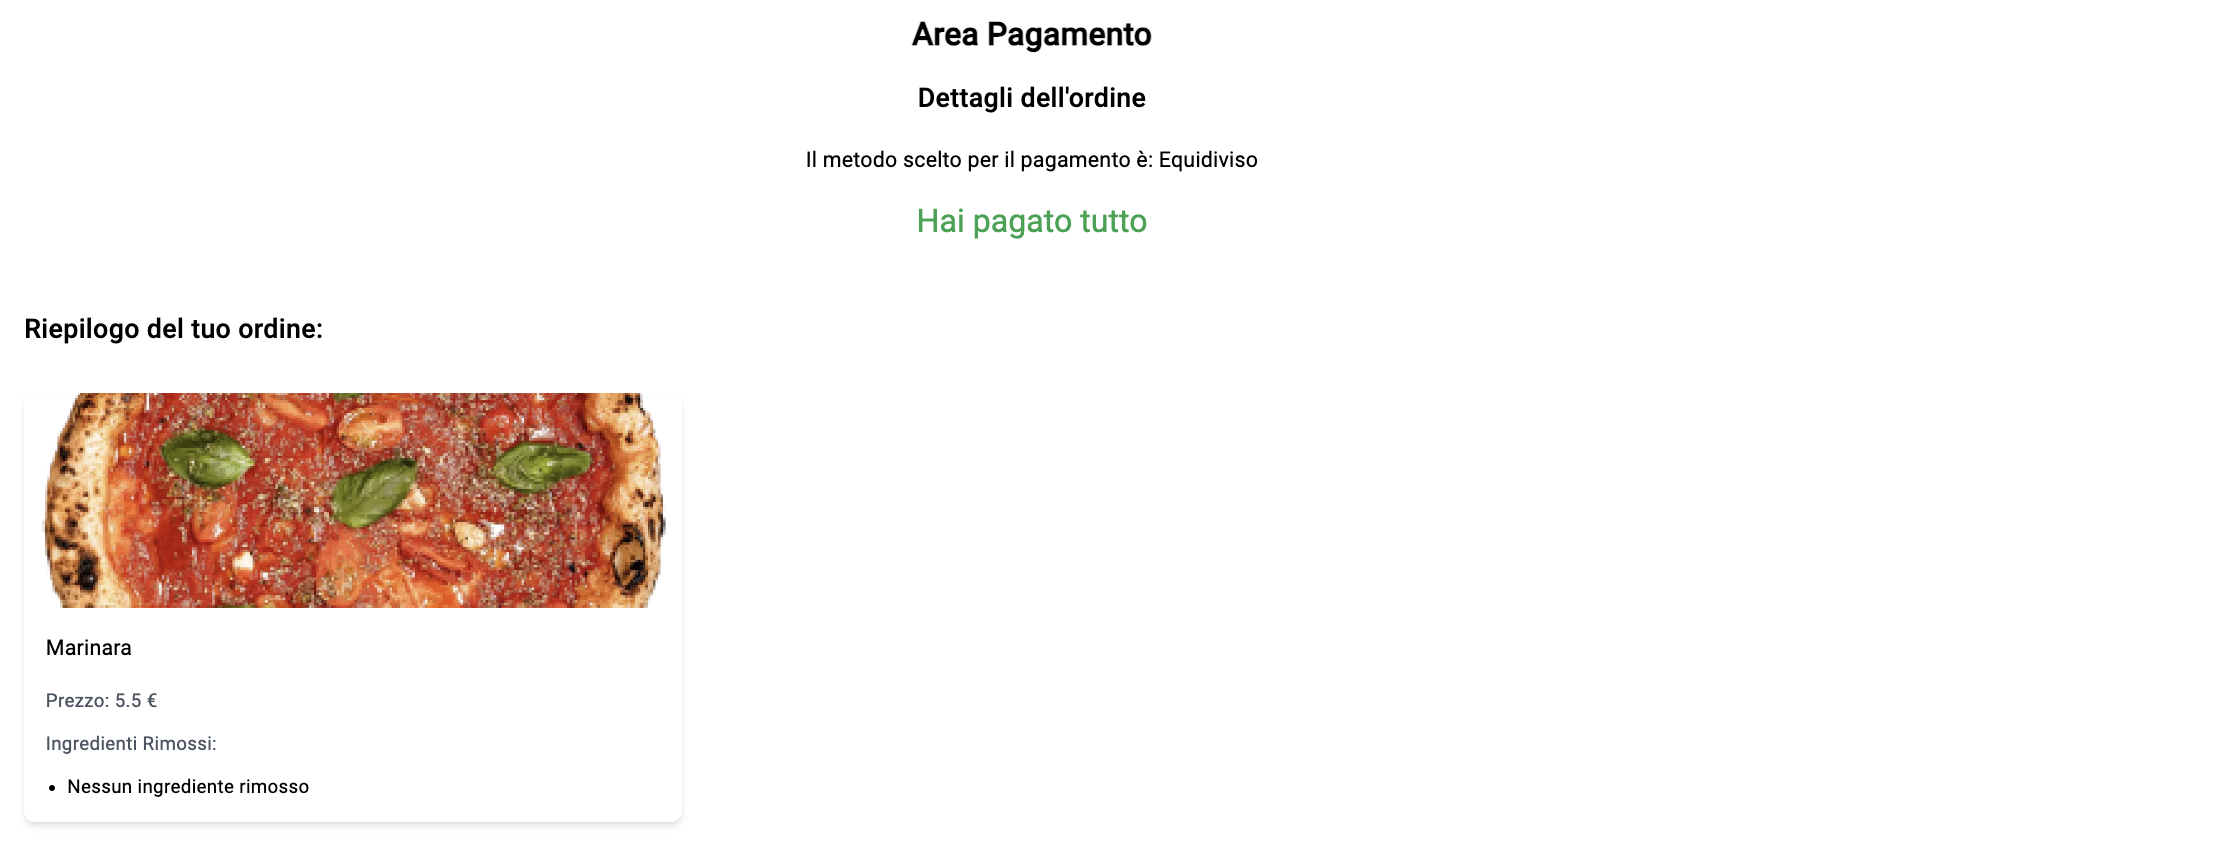
\includegraphics[width=0.8\textwidth]{PB/manuale-utente/pagamento-concluso.png}
    \caption{Pagina di pagamento concluso di una prenotazione}
\end{figure}

\subsection{Notifiche}

\begin{figure}[htbp]
    \centering
	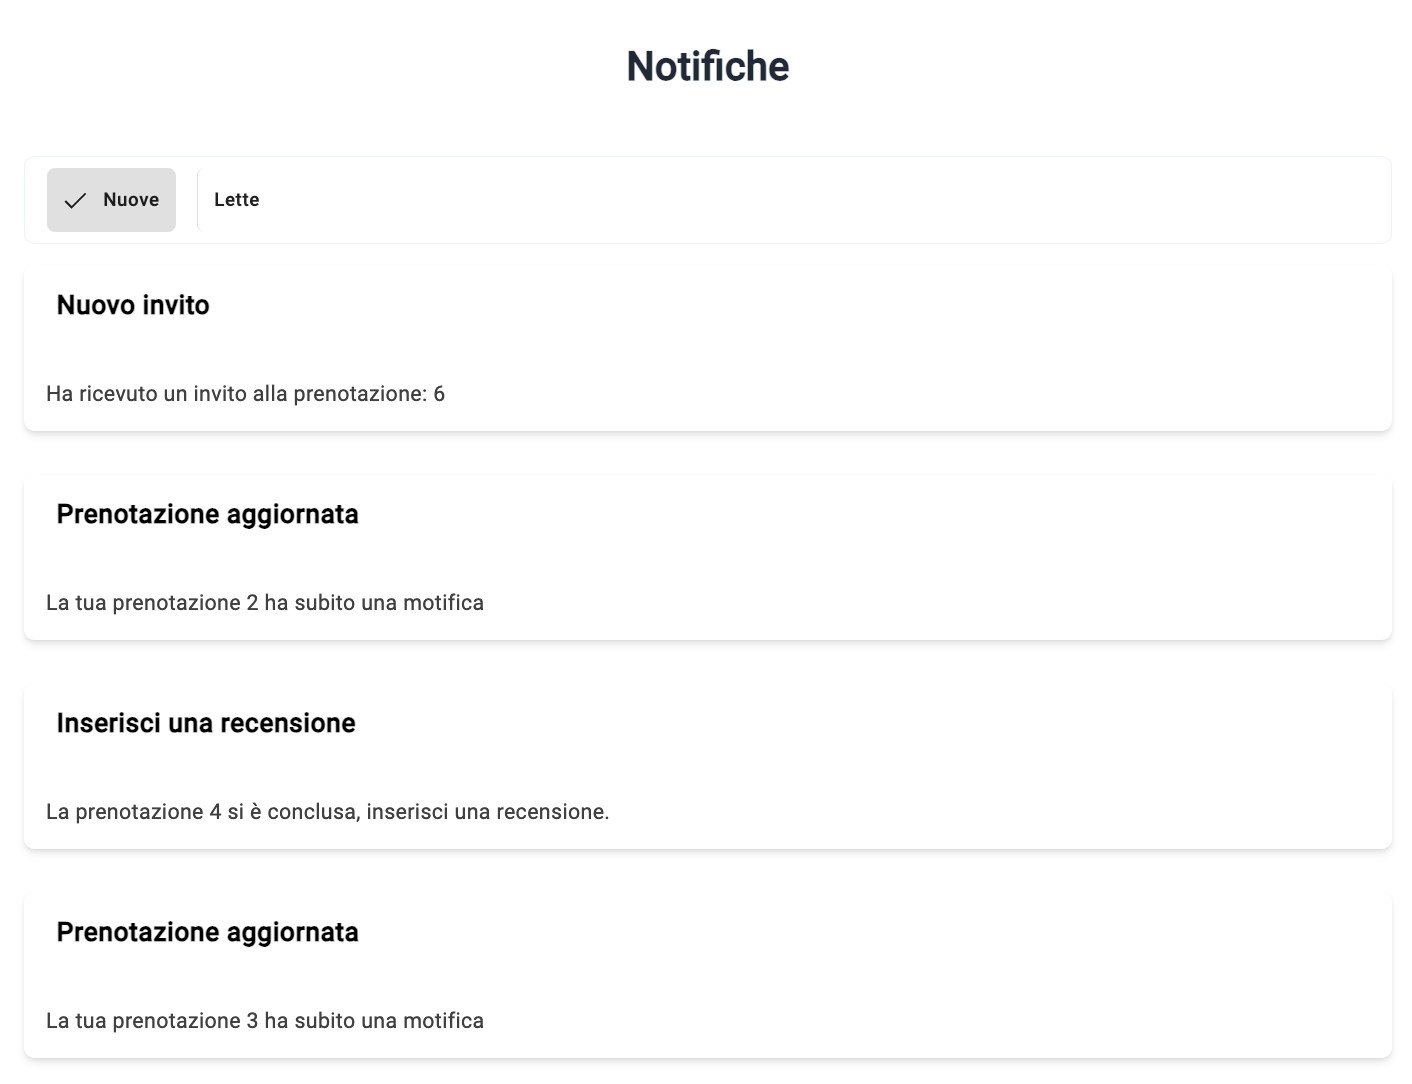
\includegraphics[width=0.8\textwidth]{PB/manuale-utente/notifiche.png}
    \caption{Pagina di pagamento concluso di una prenotazione}
\end{figure}

Si accede a questa pagina cliccando sul bottone \texttt{Notifiche} della barra di
navigazione. In questa pagina sono visualizzate tutte le notifiche di un
cliente. In cima alla lista delle notifiche sono presenti due bottoni:
\texttt{Nuove} e \texttt{Lette}. Accedendo alla pagina, è selezionato il filtro
delle notifiche nuove. Cliccando su \texttt{Lette} si visualizzano le notifiche
già lette. Passando sopra una notifica con il \textit{mouse}, compare un bottone per
segnare la notifica come letta.

\subsection{Inserimento di una recensione}

\begin{figure}[htbp]
    \centering
	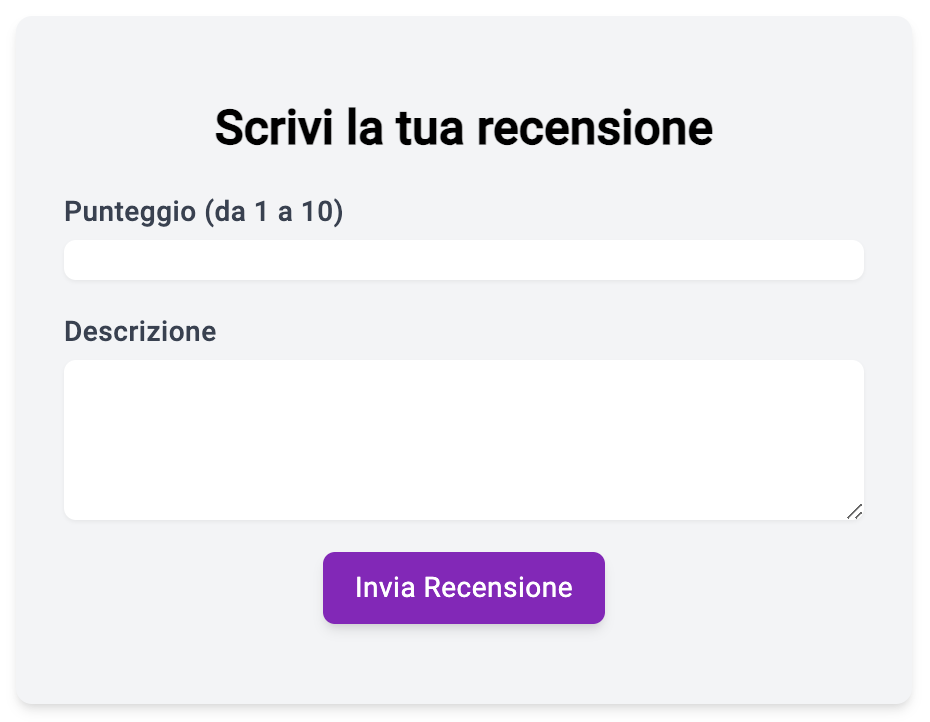
\includegraphics[width=0.8\textwidth]{PB/manuale-utente/recensione.png}
    \caption{Pagina di pagamento concluso di una prenotazione}
\end{figure}

Si accede a questa pagina cliccando sul bottone \texttt{Inserisci recensione} della
pagina di visualizzazione in dettaglio di un ristorante. Si può accedere a
questa pagina solo se si è conclusa una prenotazione e dunque si ha effettuato un pagamento presso il ristorante e non
si è ancora inserita una recensione. Dopo aver compilato il \textit{form} con le seguenti
informazioni:
\begin{itemize}
	\item Punteggio: da 0 a 10;
	\item Descrizione: una descrizione della recensione.
\end{itemize}

Cliccando sul bottone \texttt{Invia recensione} si invia la recensione. Se la
richiesta è andata a buon fine viene visualizzato un messaggio di successo. Non
è possibile modificare o eliminare una recensione una volta inviata.
